%%%%%%%%%%%%%%%%%%%%%%%%%%%%%%%
%This is the article LaTeX template for RSC journals
%Copyright The Royal Society of Chemistry 2010
%%%%%%%%%%%%%%%%%%%%%%%%%%%%%%%


\documentclass[8.5pt,twoside,twocolumn]{article}
\usepackage{}
\oddsidemargin -1.2cm
\evensidemargin -1.2cm
\textwidth 18cm
\headheight 1.0in
\topmargin -3.5cm
\textheight 22cm
\usepackage[super,sort&compress,comma]{natbib}
\usepackage{mhchem}
\usepackage{times,mathptmx}
% \usepackage{times}
% feel free not to use mathptmx if it causes difficulties
\usepackage{sectsty}
\usepackage{balance}

\usepackage{graphicx} %eps figures can be used instead
\usepackage{lastpage}
\usepackage[format=plain,singlelinecheck=false,font=small,labelfont=bf,labelsep=space]{caption}
\usepackage{fancyhdr}
\pagestyle{fancy}

\newcommand{\bra}[1]{\langle #1|}
\newcommand{\ket}[1]{|#1\rangle}

\newcommand{\be}{\begin{equation}}
\newcommand{\ee}{\end{equation}}
\newcommand{\bea}{\begin{eqnarray}}
\newcommand{\eea}{\end{eqnarray}}
\newcommand{\Fig}[1]{Fig.\,\ref{#1}}
\newcommand{\Eq}[1]{Eq.\,(\ref{#1})}
\newcommand{\la}{\langle}
\newcommand{\ra}{\rangle}
\newcommand{\nl}{\nonumber \\}
\usepackage[usenames]{color}
\definecolor{Red}{rgb}{1,0,0}
\definecolor{Blue}{rgb}{0,0,1}

\begin{document}


\thispagestyle{plain}
\fancypagestyle{plain}{
\fancyhead[L]{
\includegraphics[height=8pt]{headers/LH}}
\fancyhead[C]{\hspace{-1cm}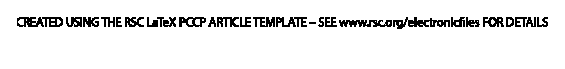
\includegraphics[height=20pt]{headers/CH}}
\fancyhead[R]{
\includegraphics[height=10pt]{headers/RH}\vspace{-0.2cm}}
\renewcommand{\headrulewidth}{1pt}}
\renewcommand{\thefootnote}{\fnsymbol{footnote}}
\renewcommand\footnoterule{\vspace*{1pt}%
\hrule width 3.4in height 0.4pt \vspace*{5pt}}
\setcounter{secnumdepth}{5}



\makeatletter
\def\subsubsection{\@startsection{subsubsection}{3}{10pt}{-1.25ex plus -1ex minus -.1ex}{0ex plus 0ex}{\normalsize\bf}}
\def\paragraph{\@startsection{paragraph}{4}{10pt}{-1.25ex plus -1ex minus -.1ex}{0ex plus 0ex}{\normalsize\textit}}
\renewcommand\@biblabel[1]{#1}
\renewcommand\@makefntext[1]%
{\noindent\makebox[0pt][r]{\@thefnmark\,}#1}
\makeatother
\renewcommand{\figurename}{\small{Fig.}~}
\sectionfont{\large}
\subsectionfont{\normalsize}

\fancyfoot{}
\fancyfoot[LO,RE]{\vspace{-7pt}
\includegraphics[height=9pt]{headers/LF}}
\fancyfoot[CO]{\vspace{-7.2pt}\hspace{12.2cm}
\includegraphics{headers/RF}}
\fancyfoot[CE]{\vspace{-7.5pt}\hspace{-13.5cm}
\includegraphics{headers/RF}}
\fancyfoot[RO]{\footnotesize{\sffamily{1--\pageref{LastPage} ~\textbar  \hspace{2pt}\thepage}}}
\fancyfoot[LE]{\footnotesize{\sffamily{\thepage~\textbar\hspace{3.45cm} 1--\pageref{LastPage}}}}
\fancyhead{}
\renewcommand{\headrulewidth}{1pt}
\renewcommand{\footrulewidth}{1pt}
\setlength{\arrayrulewidth}{1pt}
\setlength{\columnsep}{6.5mm}
\setlength\bibsep{1pt}

\twocolumn[
  \begin{@twocolumnfalse}
\noindent\LARGE{\textbf{ Quantum Chemistry Simulation on Quantum Computers: Theories and Experiments}}
\vspace{0.6cm}

\noindent\large{\textbf{Dawei Lu,\textit{$^{a}$} Boruo Xu,\textit{$^{b}$} Nanyang Xu,\textit{$^{a}$} Zhaokai Li,\textit{$^{a}$} Hongwei Chen,\textit{$^{ac}$} Xinhua Peng,\textit{$^{a}$} Ruixue Xu,\textit{$^{a}$} and
Jiangfeng Du$\ast$\textit{$^{a}$}}}\vspace{0.5cm}
%Please note that \ast indicates the corresponding author(s) but no footnote text is required.


\noindent\textit{\small{\textbf{Received Xth XXXXXXXXXX 20XX, Accepted Xth XXXXXXXXX 20XX\newline
First published on the web Xth XXXXXXXXXX 200X}}}

\noindent \textbf{\small{DOI: 10.1039/b000000x}}
\vspace{0.6cm}
%Please do not change this text.

\noindent \normalsize{It has been claimed that
quantum computers can mimic quantum systems
efficiently in polynomial scale.
Traditionally, those simulations are carried out numerically
on classical computers,
which are inevitably confronted with the exponential growth of
required resources, with the increasing size of quantum systems.
Quantum computers avoid this problem, and thus provide a possible
solution for large quantum systems.
In this paper, we first discuss the ideas of quantum simulation,
the background of quantum simulators,
categories of them, and the development
in both theories and experiments.
We then present a brief introduction to quantum chemistry
evaluated via classical computers followed by
typical procedures of quantum simulation
towards quantum chemistry. Reviewed are not only
theoretical proposals but also proof-of-principle
experimental implementations, via a small quantum computer,
which include the evaluation of the static molecular eigenenergy
and the simulation of chemical reaction dynamics.
Although the experimental development is still behind the theory,
we give prospects and suggestions for future experiments.
We anticipate that in the near future quantum simulation will become a powerful tool
for quantum chemistry over classical computations.}

\vspace{0.5cm}
 \end{@twocolumnfalse}
  ]


\section{Introduction to quantum simulation}
%Footnotes
%\footnotetext{\dag~Electronic Supplementary Information (ESI) available: [details of any supplementary information available should be included here]. See DOI: 10.1039/b000000x/}

%Please use \dag to cite the ESI in the main text of the article.
%If you article does not have ESI please remove the the \dag symbol from the title and the above footnotetext.

\footnotetext{\textit{$^{a}$Hefei National Laboratory for Physical Sciences at
Microscale and Department of Modern Physics, University of Science
and Technology of China, Hefei, Anhui, 230026, China. E-mail: djf@ustc.edu.cn}}
\footnotetext{\textit{$^{b}$King's College, University of Cambridge, Cambridge CB2 1ST, United Kingdom.}}
\footnotetext{\textit{$^{c}$High Magnetic Field Laboratory, Hefei Institutes of Physical Science, Chinese Academy of Sciences, Hefei, Anhui, 230031, China.}}
%additional addresses can be cited as above using the lower-case letters, c, d, e... If all authors are from the same address, no letter is required

%\footnotetext{\ddag~Additional footnotes to the title and authors can be included \emph{e.g.}\ `Present address:' or `These authors contributed equally to this work' as above using the symbols: \ddag, \textsection, and \P. Please place the appropriate symbol next to the author's name and include a \texttt{\textbackslash footnotetext} entry in the the correct place in the list.}


%For about thirty years since Richard Feynman
%brought forth the idea of quantum simulation
%performed inherently via quantum apparatus,\cite{Feynman}
%numerous studies have been done
%in many aspects of physics,\cite{Lewensitein}
%including in particular, quantum chemistry, materials science,
%quantum many-body problems, condensed matter physics, \emph{etc}.
%Among them, quantum chemistry,
%benefited from various theoretical approximations
%in computational simulation over the last century,
%has achieved remarkable success in
%exploring the electronic configurations of atoms and molecules,
%and interactions between them for small systems.\cite{Approximate}
%These methods, elegant and ingenious,
%ranging from wavefunction approaches to density functional theory,
%are facing challenges when the system becomes larger
%or higher accuracy is required.
%This is because the Hilbert space of quantum system
%scales exponentially with system size, making
%computational costs unfeasible within current
%classical computer architectures.
%Having realized the computational bottleneck of classical computers,
%these intrinsically quantum systems would be better simulated
%on a quantum simulator to reduce the computational
%difficulties and extract information that is inaccessible
%with classical computers.
%In this article, we first introduce the ideas of
%quantum simulations on quantum simulators
%and approaches to physical quantum simulators.
%We also briefly discuss the quantum chemistry
%and how to implement quantum simulation
%specifically for quantum chemistry problems.
%Afterwards we review the recent theoretical
%scenarios and experimental illustrations
%for some of the proposed algorithms,
%including the simulations of static molecules
%and chemical reactions.

Over the last century, quantum chemistry, benefited from various theoretical approximations
in computational simulation, has achieved remarkable success in
exploring the electronic configurations of atoms and molecules,
and interactions between them for small systems.\cite{Approximate}
These methods, elegant and ingenious,
ranging from wavefunction approaches to density functional theory,
are facing challenges when the system becomes larger
or higher accuracy is required.
This is because the Hilbert space of quantum systems
scale exponentially with system size, making
computational costs unfeasible within current
classical computer architectures.
Having realized the computational bottleneck of classical computers,
these intrinsically quantum systems would be better simulated
on a quantum simulator to reduce the computational
difficulties and extract information that is inaccessible
with classical computers.
For about thirty years, since Richard Feynman
brought forth the idea of quantum simulation
performed inherently via quantum apparatus,\cite{Feynman}
numerous studies have been done
in many aspects of physics,\cite{Lewensitein}
including in particular, quantum chemistry, materials science,
quantum many-body problems, condensed matter physics, etc.

In this article, we first introduce the ideas of
quantum simulations on quantum simulators
and approaches to physical quantum simulators.
We also briefly discuss the quantum chemistry
and how to implement quantum simulation
specifically for quantum chemistry problems.
Afterwards we review the recent theoretical
scenarios and experimental illustrations
for some of the proposed algorithms,
including simulations of static molecules
and chemical reactions.
\subsection{Advantages of quantum simulators}

The driving force in building a quantum simulator is its
advantage in solving a vast amount of problems in physics,
chemistry, and biology, together with its feasibility
within current technological development.
Classical computers
are limited to small quantum systems,
due to the huge demand of memory
and processor capability
to store and manipulate the states of large quantum systems.
This is because the number of parameters
defining the quantum states
is raised exponentially,
with respect to the increasing number of particles involved.
Moreover, the number of operations in evolving quantum states
also grows exponentially with the size of the system.
For instance, to simulate 100 spin-1/2 particles, i.e.\
the number of electrons in a moderate molecule,
a conventional computer would need $2^{100}\approx10^{30}$ bits
to describe the state,
whilst computing the time evolution is effectively
doing $2^{100}$ by $2^{100}$ matrix arithmetics.
Both requirements are beyond the capacity of current computers
and even future ones, since quantum effects would
kick in when the components in electric circuit are small enough,
leading to the upper bound on the calculating ability of
conventional computers.
However, quantum computers, in that case,
would only need 100 qubits to implement the simulation,
which is greatly fewer than $2^{100}$ bits.
Here, a qubit, a two level quantum system that is analogous
to the classical bit, is usually represented by an atom,
an electron, a photon, etc.
Thus quantum simulations on quantum computers could
not only release the potential of quantum simulation,
yielding results which are unable to calculate
on a classical circuit, but also enable us to
verify and develop theories and models,
especially on microscopic scales.\cite{Quantum_simulator}

\begin{figure}[htb]
\begin{center}
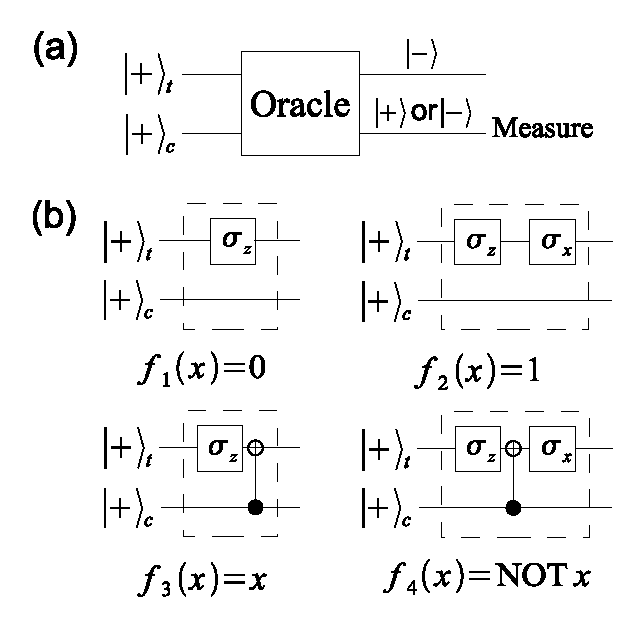
\includegraphics[width= 0.95\columnwidth]{fig1.eps}
\end{center}
\caption{(color online) Quantum phenomena describing spin-1/2 particles
from an ordered state to a random state.
For simulating this process of 45 particles with classical computers,
the memory required to store the states of the system needs
$2^{45}$ bits = $4$ tera byte (TB), which is about the current
capacity of hard disks in personal computers.
It is hard to imagine when the system scales to 100 particles
what a fantastic classical computer we need to merely store the data.
However, a quantum computer of 45 qubits is sufficient to
simulate this process. }\label{fig1}
\end{figure}

We see that quantum simulators have great advantages
over classical counterparts.
The present unperfect achievement of coherent control,
as one of the barriers to built a quantum information processer,
may soon be overcome.\cite{Coherent_control}
Therefore it is possible for the physical realization of quantum
simulation in the near future.
Additionally, unlike quantum computation which requires either
error corrections or explicit quantum gates,
quantum simulation is more feasible.
Thousands of qubits are necessary to perform a quantum algorithm,
like factorizing a modest number with Shor's algorithm,
whereas only tens of qubits are required to conduct a
useful quantum simulation.\cite{Lloyds,Alan_first,Qubits}

\subsection{Categories of quantum simulators}\label{aa}

A question comes how the quantum simulator would be implemented?
One direct method is to project the evolution of the physical system
to be simulated onto the controlled evolution of the simulating system.
Therefore, the simulating quantum system
will reproduce the physical one.
This type of device is referred
to an analogue quantum simulator (AQS).\cite{Qubits,AQS_1,AQS_2,AQS_3}
In AQS, the accuracy
depends on the resemblance between the physical system
and the simulating one. Another type of simulators,
the digital quantum simulator (DQS), is a quantum circuit,
comprised of one- and two-qubit gates
for certain unitary transformations.\cite{Lloyds,DQS_1,DQS_2}
This approach has the advantage of universality.
However, there remain challenges for the DQS,
such as the exponential growth of required gates
with the precision of the results.\cite{Quantum_simulator}
For this reason, AQS is more favored in current
quantum simulation studies,
compared to DQS, although at the end
we aim to build a universal quantum simulator.
In the following subsection, we will discuss, so far,
several (potentially) fruitful implementations of AQS
for quantum chemical applications.

\subsection{Some feasible quantum simulator architectures}

In this section, we consider some different physical systems which can be used to implement quantum simulation tasks. \cite{Nature_Rev, Rep_Rev}

$\bullet$ Nuclear Magnetic Resonance (NMR).
Since the first simulation
of quantum oscillators,\cite{NMR_oscillator}
a lot of progress has been made on this
platform.\cite{NMR_1,NMR_2,NMR_3,NMR_4,NMR_5}
Among them, in the area of quantum chemical simulations,
two proof-of-principle experiments have been done
on modeling the hydrogen molecule
H$_{2}$,\cite{NMR_static} and on simulating the
chemical dynamics of a isomerization reaction.\cite{NMR_dynamic}
In NMR architecture, nuclear spins are functioned as qubits,
and are manipulated and read-out
by an NMR spectrometer.\cite{NMR_readout}
Although the NMR system may be
limited to only few tens of qubits,
it has produced a wealth of information
and provided a testing platform
for experimental realizations of many
proposed schemes.\cite{NMR_review_1,NMR_review_2}

$\bullet$ Quantum Linear Optics. This is a more
quantum-mechanical approach than NMR ensemble,
and yet starts to show its potential in quantum computation
and quantum simulation.\cite{Optics_review_1} Indeed,
the first experiment in quantum chemistry simulation,
a minimal basis model of the hydrogen molecule H$_{2}$,
was implemented with this system.\cite{Optics_static}
Quantum optics system relies on the different degrees of freedom (DOF)
of single photons, i.e.\ polarizations and paths,
as qubits to encode quantum
information.\cite{Optics_review_1,Optics_review_2}
It is regarded as an available platform for
quantum chemical simulations, despite challenges remaining in
hardware, e.g.\ the reliability of output and detection
of a number of coherent single photons.\cite{Optics_first}

$\bullet$ Trapped Ions. As one of the most controllable systems
available today, many advanced physical systems,
such as quantum magnet and Dirac equations,
have been simulated on this
platform.\cite{Qubits,Ions_expt_2,Ions_expt_3}
For this structure, qubits are represented by the electronic states
of cold trapped ions.\cite{Ions_review_1,Ions_review_2,Ions_review_3}
However, chemical simulations are yet to be realized.

$\bullet$ Superconducting Circuits. Besides synthesizing arbitrary states and implementing simple 2-qubit algorithms in experiment,\cite{Super_1,Super_2} superconducting circuits are supposed to simulate phenomena in atomic physics,\cite{Super_3,Super_4} realize the Kitaev model on a honeycomb lattice,\cite{Super_5}, emulate large-spins,\cite{Super_10} or simulate the Anderson and Kondo models.\cite{Super_6,Super_11} The flowing circulating current in a superconductor can be used as a qubit.\cite{Super_7,Super_4,Super_8,Super_9} Precise control and measurement in this system has been demonstrated, but the scalability problem remains to be solved.

$\bullet$ Quantum Dots. The electron spins in semiconductor quantum dots with discrete energy levels,\cite{Dot_1} which are analogous to a real atom binding an electron, have been proved to simulate the Fermi-Hubbard model\cite{Dot_1,Dot_2} and the many-fermion problem in high-Tc superconductors.\cite{AQS_2} A feasible proposal has also been brought forward to model chemical reactions.\cite{AQS_3}

$\bullet$ Cold Atoms. Neutral atoms in optical lattices are important potential quantum simulators, especially for condensed matter physics. The simulation of the quantum phase transition was first implemented in this system, realizing a superfluid transferred to a Mott insulator.\cite{AQS_1} Numerical examples that could be simulated are discussed in the review paper by Lewenstein,\cite{Lewensitein} while experimental approaches can be found in Bloch's paper.\cite{Cold_1}

\section{Quantum chemistry}

\subsection{Classical approach to quantum chemistry}

Quantum chemistry aims at developing theoretical methods
to calculate molecular properties and evolutions
on the basis of quantum mechanics. Most quantum chemical approaches
involve the Born-Oppenheimer approximation to separate
electronic and nuclear motions. However, even in this frame,
exact solution of the Schr\"{o}dinger equation
requires the computational resources increase exponentially
with the molecular size. Because of this, the developments of
quantum chemical methods have always
adopted various approximations.

The first important task of quantum chemistry is to
study static molecular properties, such as
electronic structures and eigenenergies,
vibrational normal modes, etc.
Methods in this aspect include the mean-field
Hartree-Fock and various post-Hartree-Fock approaches
for the electronic correlations,
such as the configuration interaction,
coupled cluster, and many-body perturbation
theories.\cite{Hydrogen}
These high-precision calculations can only be
performed on very small molecular systems.
Density functional theory\cite{Parr95,Kohn96,Chelikowsky09}
has a relatively high efficiency and enlarges the system size
of application with a certain accuracy.
Linear scaling algorithms\cite{Hung09, Goedecker99} are also
developed to explore systems of thousands of atoms or even larger
for certain typies of materials.
These methods can sometimes predict chemical properties
for large systems, but in some cases they may fail.\cite{Yang08,limit_1,limit_2,limit_3}



\iffalse


  For the time-independent Hamiltonian, the exact solution of the Schr\"{o}dinger equation requires the computational resources increase exponentially with the molecular size scaling. Although the most important task in quantum chemistry is to calculate the energy spectrum of fixed molecules to a required accuracy, such tasks for exact calculations must be limited in small systems in classical computers for the complexity reason. Several approximate methods have been developed to solve this problem, such as density functional theory (DFT) calculations.\cite{DFT_1,DFT_2} These methods can sometimes predict chemical properties for larger systems, but in some cases they will fail.\cite{limit_1,limit_2,limit_3}


\fi



Another important task in quantum chemistry is
the simulation of chemical dynamics,
not only to explore the reaction mechanisms
but also to guide the control of
chemical reactions.\cite{Reaction_1,Reaction_2}
Using conventional methods without approximations,
the capacity of investigating chemical reaction dynamics
so far is just 9 DOF.\cite{DOF}
Even the multiconfigurational time-dependent
Hartree method,\cite{Hartree} which is highly sophisticated
with various approximations and models,
can just deal with tens of DOF.
Similarly as in the static case,
to simulate quantum dynamics of large molecular systems
is currently intractable using classical computers.

\subsection{Typical procedure of quantum simulation towards quantum chemistry}

We have introduced the backgrounds for quantum simulation,
quantum simulator, and quantum chemistry.
In this section, we will discuss approaches used in quantum simulation.
Specifically, we will focus on the methods and techniques applied
in quantum chemistry simulations, especially those which have been
or are likely to be implemented in the near future.

In quantum simulation, we are interested
in  the behavior and properties of a quantum system,
which could be either a stationary molecule or a chemical reaction.
The procedure of quantum simulation
can be summarized in three steps:
a) preparing the quantum state into an initial state,
b) evolving the initial state with the system Hamiltonian, and
c) measuring the desired properties from the final state.

Before we move on to discuss each of these steps,
we recall that the
two major schemes in quantum simulation
are digital (universal) quantum simulation (DQS)
and analogue (dedicated) quantum simulation (AQS).
As mentioned in Section \ref{aa},
currently most research groups concentrate on AQS
instead of DQS due to the difficulty in performing a DQS.
Therefore, the arguments below will mainly apply to AQS,
although some of them could also be used on DQS.
%which will be addressed accordingly.

\subsubsection{Preparing the quantum state into an initial state.}

\iffalse
It is costly to simulate arbitrary dynamics.
Fortunately natural systems are not arbitrary\cite{Lloyds}
and hence chemical simulation can be done efficiently.
\fi
In principle, there are two ways to
simulate a chemical system.\cite{Simulating_chemistry_computer}
One is the second quantization method where the
Born-Oppenheimer approximation is adopted.
It considers that electrons in a molecule
are indistinguishable, unlike individually identifiable qubits.
The advantage of this approach is that
it is economical with quantum resources,
as it requires only one qubit per basis.
Due to this, the first quantum chemical experiment
was performed using this method.\cite{Optics_static}
Nonetheless, this method is not suited
if the system is complex and cannot be
represented by a small basis set,
or if it is a dynamic
problem which cannot be associated with a fixed basis set.
To overcome this, people also introduce the first quantization method.

The first quantization approach does not take into account
the Born-Oppenheimer approximation.
Instead, it simulates particles altogether
including both nuclei and electrons
governed by the Schr\"{o}dinger equation
on a grid in real space.\cite{first_quantization_1,first_quantization_2,Polynomial_time_algorithm}
Although it may need an excessive amount of resources
compared to the second quantization,
it has advantages when the system becomes large.
Since the Coulomb interaction is operated in
different representations,
the second quantization method requires $O(P^5)$ gates where $P$
denotes the size of the basis set,
while using the first quantization approach the number of gates
scales at $O(Q^2)$
for a $Q$-particle system.\cite{Polynomial_time_algorithm,Simulating_chemistry_computer}
It is found that the first quantization scheme will be
more efficient to simulate reactions
of more than four atoms.\cite{Polynomial_time_algorithm}

%The above methods are universal in terms of preparing initial states and propagating with time. However, to date, the only experimental implementations of quantum chemical simulation involving initialization were on NMR systems. Therefore, we would like to address the techniques in NMR simulator for preparing initial states.

%For most quantum simulations, a pure initial state is required, for instance, electrons with all spin-up or spin-down. However, a theoretical breakthrough was made on NMR systems, that allow to prepare effective pure or pseudo-pure states from thermal states at room temperature \cite{pseudo-pure},\cite{logical_labeling_1},\cite{spatial_averaging_1}. So far, three primary methods have been developed for this process: logical labeling \cite{logical_labeling_1}\cite{logical_labeling_2}, temporal averaging \cite{temporal_averaging_1}, spatial averaging \cite{spatial_averaging_1}. However, the last two approaches have been the most popular choices, to date. And actually the first realization of chemical simulation on NMR adopted the spacial averaging method to prepare the effective pure states\cite{NMR_static}.

%In quantum chemical simultion, the last step for preparing the initial state from the pure state is usually via adiabatic computation\cite{Adiabatic_1}. In this model, the state stay in its ground state throughout the procedure, and the Hamiltonian varies slowly from the effective pure state to the desired initial state(see \cite{Adiabatic_2}\cite{Adiabatic_3}\cite{Adiabatic_4}\cite{Adiabatic_5}).

\subsubsection{Evolving the initial state with the system Hamiltonian.}

\ Currently, we select the Trotter formula\cite{first_quantization_2}
and its generalization in high dimensions\cite{Trotter_1,Trotter_2}
to generate the unitary evolution
of a system Hamiltonian that is to be simulated. Assume that the system Hamiltonian can be written as $H = \sum_{m=1}^MH_m$,
where $H_m$ is local interaction Hamiltonian. The unitary operator of the evolution would be $U(t) = e^{-iHt}$, whose decomposition is usually difficult.
By using the first-order Trotter formula and small time intervals $\delta t \rightarrow 0$,
\begin{eqnarray}\label{trotter}
 U(\delta t) & = & e^{-iH\delta t} = \prod\limits_{m=1}^M e^{-iH_m\delta t}+\mathcal {O}(\delta t^2)\nonumber \\
 & \approx & \prod\limits_{m=1}^M e^{-iH_m\delta t}.
\end{eqnarray}
Noting that the accuracy of this formula can be improved by choosing very small $\delta t$ or choosing higher-order decompositions, both of which will produce a large number of logical gates and accumulate the errors due to the imperfection of each gate in experiment.

%Essentially, this formula decomposes the time period
%in the propagator into small time intervals.
%The desired evolution is implemented
%by iterating the process of each step.

\subsubsection{Measuring the desired properties from the final state.}

\ There are mainly two methods that have been used in
experiments to obtain information from the final state.
The first one, quantum state tomography, can fully
characterize the final state after its evolution.
However, the required resources grow exponentially
with the size of the state since it reads out the whole
Hilbert space of the state. Nevertheless, it provides a valuable method
to evaluate the fidelity of the final results
for low-dimensional states, especially in those proof-of-principle experiments.
Another type of read-out technique is called
phase estimation algorithm (PEA).\cite{PEA_1,PEA_2,PEA_3,PEA_4}
Often the information of the state is encoded in the global phase
which is of no use, as it is not observable.
Using the PEA, the information is transferred to the ancilla qubits
and extracted from the latter by performing measurements on the latter.
The scalability of this method is universal.
However, the demand for extra ancilla qubits
restricts it from wide use in circuit.
As it is known, to date, it is still a technical challenge
to generate and manipulate many qubits in any quantum structure.
So far, the two experimental realizations of static molecular modeling
are performed via an improved version of
the PEA.\cite{Optics_static,NMR_static}
Essentially, by iterating the PEA process
and modifying the parameters, i.e.\
the pulses in the circuit, accordingly,
high-precision results can be achieved.
However, another experiment,\cite{NMR_dynamic}
which was on simulating chemical dynamics,
turned to quantum state tomography as its measurement technique.
It was effective in that experiment
since only three qubits were involved
and the associated Hilbert space was small enough.
Additionally, quantum tomography provided a direct way
to reconstruct the final state and to calculate the fidelity
of the results. Nevertheless,
this method could not be conducted when the system scales up,
for the reason discussed above.
The PEA and other approaches\cite{Other_measuring_methods_1,Other_measuring_methods_2,Other_measuring_methods_3,Other_measuring_methods_4}
would be the promising methods for measurements
when systems contain tens of qubits or more.

\section{Simulation of static molecular energies}

\subsection{Theoretical designment on simulating the molecular ground state energies}

In a quantum system,
the most fundamental properties are its
energy eigenvalues and eigenstates.
Accurate calculations of them request a quantum algorithm.
This is the same situation as in quantum chemistry,
where given a time-independent Hamiltonian of a molecule,
the first task is to calculate the ground state energy, i.e.,
the lowest eigenvalue of the Hamiltonian.
In classical computers, it is a non-deterministic polynomial (NP) problem.
All known classical algorithms for it require exponential time.
On the other hand, quantum algorithm or quantum simulation
is theoretically proved to be able to solve this problem efficiently,
in polynomial time.\cite{PEA_1}
With the help of quantum fast Fourier transform (FFT),
the eigenvalues and eigenstates of a local Hamiltonian
can be solved in polynomial time.
Abrams and Lloyd\cite{PEA_1} believed that many interesting problems
in atomic physics which are classically intractable
can be solved with 50 to 100 qubits.
This means that quantum computers in this size
would surpass the capacity of classical computers.
Recently, Li \emph{et al.}\cite{Li}
employed a trial wavefunction, approximating the ground state,
to project the ground state by means of the PEA,
and performed an NMR experimental implementation of this idea
to solve the ground-state problem
of the Heisenberg spin model.
Concerning the static properties of a molecule in quantum chemistry,
Aspuru-Guzik \emph{et al.}\cite{Alan_first} proposed an algorithm
to calculate the energies of molecules in 2005.
Compared to the previous algorithms,
the information of eigenenergy in their work
is encoded in the phase shift,
and measured by a recursive PEA which
reduces the number of qubits constituting the readout register
from 20 to 4.
In this scheme, the number of qubits scales linearly
with the number of basis functions,
and the number of gates scales polynomially,
because the direct mapping from wavefunctions to qubits
ensures the whole unitary operator
be decomposed into a polynomial number of quantum gates.
They conclude\cite{Alan_first} that quantum simulation
with 30 to 100 qubits can exceed the limitations
of classical computing. %repetition


The main procedure of simulating molecular energies can be summarized into three steps:

(i)\emph{ Encoding and initialization.}
All quantum simulation tasks require a proper mapping
from the system wavefunction to the state of qubits,
to establish a bridge between the simulating system
and physical system. The wavefunctions of many-particle systems
are often represented by single-particle atomic orbits,
which also depend on the choice of basis sets.
There are essentially two different mapping methods:
direct mapping in which a Fock space of the molecule
is mapped onto the Hilbert space of the qubits,
and more efficiently, the compact mapping,
in which only a subspace of the Fock space
is mapped onto the Hilbert space.
For instance, to map the wavefunctions of water,
with the simplest STO-3G basis set including 7 wavefunctions,
the direct and compact mapping methods require 14 qubits
and 10 qubits, respectively. If we choose
the cc-pVTZ basis set including 58 wavefunctions,
the two maps would need 116 and 47 qubits, respectively.\cite{Alan_first}
The resources required exceed the experimental
capacity in current quantum simulations,
whereas it would be more possible to realize in the near future,
compared to conventional quantum algorithms
which usually need thousands of qubits.

To prepare the initial state, i.e.,
the ground state $|\psi\rangle$ of a molecular Hamiltonian,
the adiabatic state preparation (ASP) algorithm,
using the quantum adiabatic theorem,\cite{adiabatic}
is a suitable approach. The quantum adiabatic theorem states that,
a quantum system remains in its instantaneous eigenstate,
if the system Hamiltonian varies slowly enough,
and if there is a gap
between this eigenvalue and
the rest of the Hamiltonian's spectrum.\cite{adiabatic}
Therefore we can choose a simple Hamiltonian
and prepare the state according to its ground state.
We then drive the simple Hamiltonian
to the target molecular Hamiltonian sufficiently slowly,
in which all the energy levels are ensured to be noncrossing.
After the adiabatic process, the qubits
have been prepared to the initial state,
the ground state of the molecular Hamiltonian.

(ii)\emph{ Evolution.} The core of the evolution is
the implementation of the PEA to generate a phase shift
on the probe qubit which reflects the information
of the target eigenvalue.
Briefly, applying $U=e^{-iH\tau}$ on the ground state
$\left\vert \psi \right\rangle$, a phase will be induced
on the exponential term $U \left\vert \psi \right\rangle =
e^{-iH\tau}\left\vert \psi \right\rangle =
e^{-iE\tau}\left\vert \psi \right\rangle =
e^{i2 \pi \phi}\left\vert \psi \right\rangle$,
where $E=-2\pi\phi/\tau$ is the eigenvalue of the ground state.
Experimentally, we confine the phase $\phi$ between zero and unity
by a pre-estimated value of the energy $E$.
If the phase on the probe qubit can be
measured with high accuracy, the resulting eigenvalue
would be very precise,
surpassing the results reached by
the classical computers. However, this will cost
many qubits in resource.

To overcome this, a modified PEA is proposed\cite{Alan_first}
to reduce the number of qubits.
The main idea is a recursive PEA,
which repeats an arbitrary $n$-qubit PEA
using $V_{k+1}=[e^{-i2 \pi \phi_k}V_k]^2$.
Here $\phi_k$ is a lower bound on the constructed shift $\phi$ at
each iterative step $k$.
The initial condition is $V_{0}=U=e^{-iH\tau}$.
In each step, one additional bit of $\phi$ is obtained,
and a long enough digit can be achieved
by repeating this procedure many times.
No matter how small the number of qubits $n$ is
(even only one qubit), accurate results can be obtained
as long as the iterations of PEA are carried out enough times.

(iii)\emph{ Measurement.}
Since the ground state energy has been encoded
in the phase of the probe qubits,
a direct measurement of this phase is sufficient
to obtain the value of the ground state energy. For example,
if a four-bit inverse quantum Fourier transform is adopted
for the phase measurement,
we will need four qubits
to obtain one precise bit with successful possibility of 15/16.%\cite{Alan_first}
%Full state tomography of the probe qubits, which extracts all the data of the logical state, is obviously able to accomplish the task. However, tomography is not proved to be a scalable method for reading out quantum states, which might be useless for simulating large molecules. Other readout methods, such as the interferometer

Similar to other quantum simulation tasks,
in the field of chemical simulations,
theory is still ahead of experiments.
The present experimental technology cannot support the simulation of large molecules,
whereas proof-of-principle experiments are available
using current quantum simulation devices.
As the first and key exemplification of quantum simulation
towards quantum chemistry, the simplest but most
significant scenario for simulating the ground state energy
of the hydrogen molecule is a good choice.
The first two experiments both selected
this problem, using a linear optical system\cite{Optics_static}
and an NMR system,\cite{NMR_static} respectively.
We will review these two experiments briefly in the following section.

\subsection{Experiments for simulating the ground state energy of the hydrogen molecule}

%In 2010, Lanyon \emph{et al.}\ demonstrated the quantum simulation
%of molecular eigenenergies using a linear optical quantum
%computation architecture for obtaining the energies
%of the hydrogen molecule in a minimal STO-3G basis.\cite{Optics_static}
In 2010, it was demonstrated that the ground state energies of the hydrogen molecule in a minimal STO-3G basis could be simulated using a linear optical quantum
computation architecture.\cite{Optics_static}
In the linear optical system,
quantum information is encoded in polarization
or path of single photons.\cite{Optics_review_1,Optics_review_2}
In the experiment, two qubits were utilized to
implement the simulation, with one to encode the system wavefunction,
while another to read out the result of the PEA.
For each iterative process, one bit precision was obtained.
The whole iterative PEA was repeated for 20 times,
achieving a high level of 20 bit precision in total.
%The experimental result matches exactly
%with the theoretical calculation
%and promises the chemical application of quantum simulation.
%Despite the other steps of the algorithm
%are assisted by a classical computer,
%the key step of performing the iterative PEA
%is realized perfectly on a linear optical quantum system,
%yielding important progress towards simulating quantum chemistry.
The key step of performing the iterative PEA was realized on a linear optical quantum system, and 
the other steps of the algorithm including initial state preparation were assisted by a classical computer.
The authors discussed how the technique could be expanded to solve large-scale chemical problems that lie beyond
the reach of modern supercomputers, and claimed that the experimental results represented an early practical step toward a powerful tool with a broad
range of quantum-chemical applications.



\begin{figure}[htb]
\begin{center}
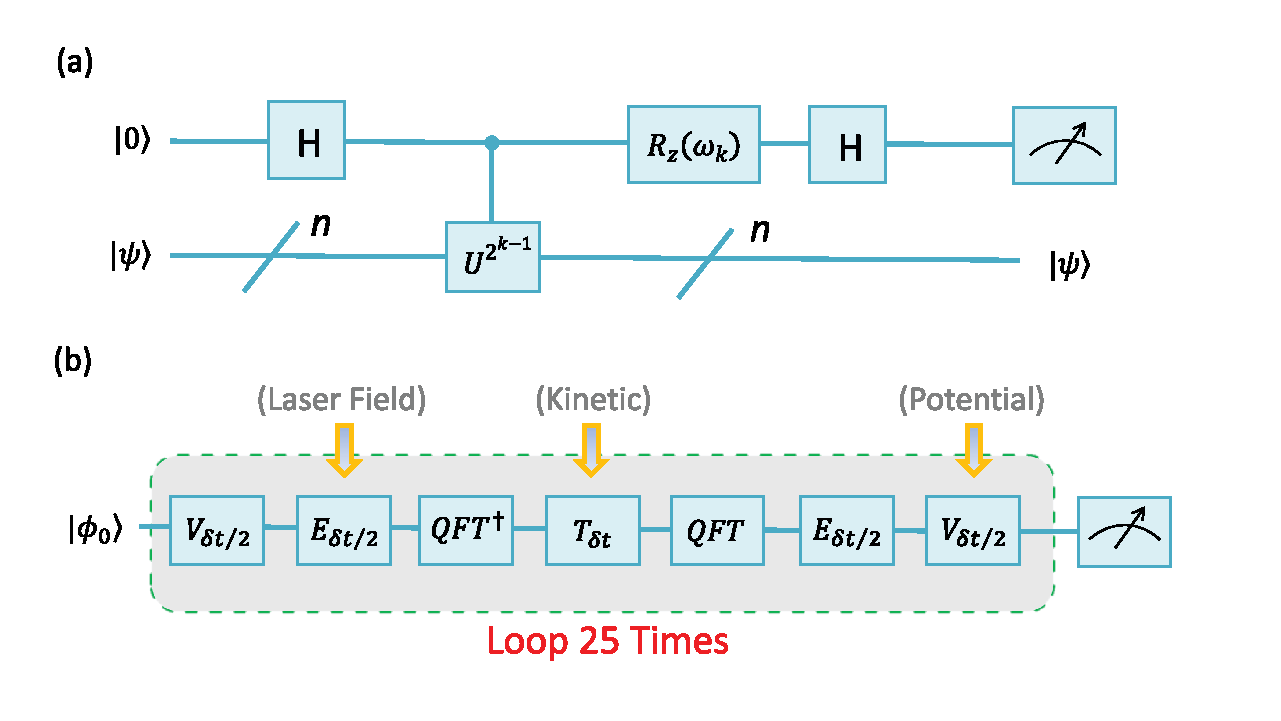
\includegraphics[width= 0.95\columnwidth]{fig2.eps}
\end{center}
\caption{(color online) (a) Network of the iterative phase estimation algorithm
for the calculation of the hydrogen molecular energies. Reproduced from Lanyon  \emph{et al.}, \emph{Nat. Chem}., 2010, \textbf{2}, 106-111.\cite{Optics_static}
(b) Network of simulating the isomerization dynamics from
the reactant state $\left\vert \phi_{0} \right\rangle$ where
the whole process is divided into 25 loops. Reproduced from Lu  \emph{et al.}, \emph{Phys. Rev. Lett.}, 2011, \textbf{107}, 020501.\cite{NMR_dynamic}}\label{fig2}
\end{figure}

The Hamiltonian of the hydrogen molecule in the minimal STO-3G basis
was block-diagonal with 2 $\times$ 2 submatrices,
conducing one qubit to represent the system wavefunction
and another to represent the phase information.
Exact eigenstates were first encoded,
which were preliminarily calculated through a classical computer.
For imperfect eigenstate encoding,
the algorithm was robust and still works well.
The quantum state $\left\vert 0 \right\rangle$ and
$\left\vert 1 \right\rangle$ were represented via
the horizontal and vertical polarization
$\left\vert H \right\rangle$ and $\left\vert V \right\rangle$,
respectively.
A single rotating gate was implemented using birefringent wave plates,
and a two-qubit gate was implemented by combining the phase shifters
and beam splitters with projective measurement.
The quantum circuit model can be found in Fig.\ref{fig2}(a).
The ground state energy was obtained as -535.58 $\pm$ 0.03 kJ mol$^{-1}$,
which agrees well with the result calculated
from a classical computer.

Almost simultaneously to the optical experiment, the proposal of
simulating the ground state energies of hydrogen molecule was
demonstrated via an NMR system.\cite{NMR_static}
The basis was selected as the widely used minimal STO-3G as well,
and a two-qubit sample of $^{13}$C-labeled chloroform dissolved
in $d_6$ acetone was employed in the NMR spectrometer.
Qubits were represented by $^{13}$C (system qubit) and
$^{1}$H (probe qubit)
nuclear spins. ASP \cite{factoring} was tested for various bond
distances, with $r=1.4$ a.u.\ being found the most suited to be used to
prepare the initial state,
i.e., the ground state of the hydrogen molecule in the minimal basis.
A 15-step iterative PEA process was implemented as the essential part of
the algorithm, with a 3-bit precision extracted per iteration,
achieving a 45-bit precision. The readout was performed
through an NMR interferometer,\cite{inter1,inter2,inter3} to obtain
the phase shift of the probe qubit.
The experimental result of the ground state energy is exact,
with the uncertainty being only in the last and also the least
important bit.

Considering the singlet symmetry and spatial symmetry, the Hamiltonian of the hydrogen molecule in the STO-3G basis could be simplified as\cite{Hydrogen}
\begin{eqnarray}
        H&=&
        \begin{pmatrix}
            \langle\Psi_0|H|\Psi_0\rangle & \langle\Psi_{1\bar{1}}^{2\bar{2}}|H||\Psi_{1\bar{1}}^{2\bar{2}}\rangle\\
            \langle\Psi_{1\bar{1}}^{2\bar{2}}|H|\Psi_0\rangle & \langle\Psi_{1\bar{1}}^{2\bar{2}}|H|\Psi_{1\bar{1}}^{2\bar{2}}\rangle
            \end{pmatrix}\nonumber\\
        &=& \begin{pmatrix}
            -1.8310 & 0.1813\\
            0.1813 & -0.2537
            \end{pmatrix},
\end{eqnarray}
whose eigenvalue is -1.85157092935119 a.u. Here this eigenvalue was given with 15 significant figures to show the contrast between the theoretical value and experimental value clearly.
Spin $^{13}$C was used to modulate the system Hamiltonian.
In NMR architecture, the logical states $\left\vert 0 \right\rangle$
and $\left\vert 1 \right\rangle$ were represented by the nuclear
spin up $\left\vert \uparrow \right\rangle$ and
spin down $\left\vert \downarrow \right\rangle$, respectively.
A single rotating gate was realized by applying short accurate hard
pulses for arbitrary angles and a two qubit gate was realized
by modeling the free evolution of the NMR internal Hamiltonian
combined with the decoupling technique.\cite{NMR_review_1}
The whole experiment was divided into three parts:
the adiabatic preparation of the system qubit $^{13}$C to
the ground state of the Hamiltonian; the application of the
controlled evolution of the Hamiltonian
to produce a phase shift on the probe qubit;
and the measurement of the phase shift to obtain
the value of the ground state energy.
The network and the corresponding pulse sequence were
displayed in Figure 1 of Du's paper.\cite{NMR_static}
Instead of taking tomography of the probe qubit,
an NMR interferometer equipment was utilized to measure
the phase shift accurately, since the error bound of it
was less than $\pm 5^{\circ}$. After 15 iterations the ground
state energy of the molecular Hamiltonian was extracted as
 -1.851570929351124 a.u.
The intermediate results after each iteration are
shown in Fig.\ref{fig3}.

\begin{figure}[htb]
\begin{center}
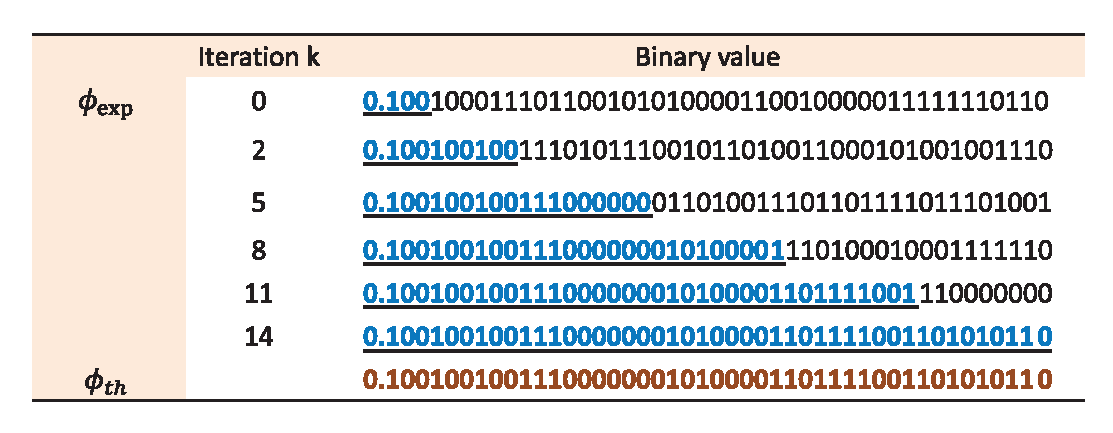
\includegraphics[width= 0.95\columnwidth]{fig3.eps}
\end{center}
\caption{(color online) Experimental $\phi$ values ($\phi_{exp}$) measured in iterations, compared to the theoretical
expectation $\phi_{th}$ (brown). The numbers with underlines are the bits obtained from the experiment, where 3 bits are
extracted in each iteration. Through 15 iterations,
we ultimately obtain 45 bits of $\phi$, whose value is exactly the same as the theoretical result. These results are from Du \emph{et al.}, \emph{Phys. Rev. Lett}., 2010, \textbf{104}, 030502.\cite{NMR_static}}\label{fig3}
\end{figure}

The overview of the two proof-of-principle experiments
lead us to consider larger molecular size and scale the
algorithm to carry out complicated simulations of
molecular energies that are impossible via classical computers.
We conclude that the dream may come true if the following two difficulties
can be overcome in the future. One is the more
efficient decomposition of the evolution operator
of the molecular Hamiltonian and the other is
the complexity of the ASP.
For the first issue, an overview of the operator-splitting
technique is given in the supplementary material of Lanyon's paper.\cite{Optics_static}
They find that the number of the quantum logical gates
decomposed to simulate an arbitrary molecule is $N^5$,
where $N$ is the number of involved single-particle basis functions,
which is also the number of necessary qubits.
On the second issue, some numerical simulations of the adiabatic
evolutions have been performed showing a polynomial growth
with the system size up to 128 qubits,\cite{Adiabatic_6}
and the polynomial time complexity has also been analytically obtained
when the adiabatic evolution is performed to
have phase transitions of second or higher orders.\cite{Adiabatic_7}
Thus, when the necessary hardware and technical difficulties
are overcome, the quantum simulation of ground state energies
of medium-size molecules is feasible in principle.

\section{Simulation of chemical reaction dynamics}

\subsection{Theoretical designment on simulating chemical reaction dynamics}

Having discussed experiments on
static molecular energy simulations,
we now concentrate on the second important task in quantum chemistry,
the simulation of chemical dynamics.
It is a fundamental problem in quantum chemistry
to understand and analyze the mechanism of chemical reactions.
As discussed above, the main obstacle of quantum dynamics simulation
by classical computers is the exponentially required resources
with the size of the system.\cite{Open_Dynamics} This makes simulating a dynamic process
more difficult than simulating a stationary model,
because a dynamic process involves more atoms and molecules
and hence has greater complexity.
%Nonetheless, in 2008, Kassal \emph{et al.}\
%proposed an algorithm (DQS) which could reduce this problem
%to be a polynomial complexity one on quantum computers.\cite{Polynomial_time_algorithm}
Nonetheless, in 2008, an algorithm (DQS) was proposed to reduce this problem
to be a polynomial complexity one on quantum computers.\cite{Polynomial_time_algorithm}
They adopted the first-quantization methods
which directly simulates electronic and nuclear interaction
evolving in time without applying
the Born-Oppenheimer approximation.
It turns out that this approach is more efficient
on a quantum computer than on a classical computer,
when the number of atoms in the reaction is more than 4.

In their algorithm, they represent the system by
wavefunctions in coordinate representation,
which are discretized with qubits.
For simplicity, the Hamiltonian is assumed to be time-independent,
and the potential only depends on position.
In other words, $\hat{H}$ = $\hat{T}$ + $\hat{V}$,
where $\hat{T}$ = $\hat{p}^{2}$/2$m$ and $\hat{V}$ = $V(\hat{x})$
are the kinetic and potential energy operators, respectively.
In practice, the split-operator technique\cite{first_quantization_2,Trotter_1,Trotter_2}
is applied to decompose the propagator $\hat{U}(t)$
into contributions from the kinetic $\hat{T}$ and potential $\hat{V}$
components separately, which are discussed in Section 4.2 in detail.
%For a sufficiently small time interval $\delta t$,
%the propagator $\hat{U}$ could be separated,
%up to first-order in $\delta t$, as
%\[\hat U(\delta t) = {e^{ - i\hat H\delta t}}
%= {e^{-i\hat T\delta t}}{e^{-i\hat V\delta t}} + O(\delta {t^2})\]
%From now on, we set $\hbar=1$.
%Undoubtedly, using a higher-order decomposition
%of the propagator\cite{Trotter_1,Trotter_2}
%would increase the accuracy of this implementation.

It is noticed that the operators $e^{ - i \hat{T} \delta t}$
and $e^{ - i \hat{V} \delta t}$
are diagonal in the momentum and coordinate representations, respectively.
They can be transformed easily from one to another
via the quantum Fourier transformation (QFT)\cite{QFT_1}
on a quantum computer,
\[|\psi (t+\delta t)\rangle  = \hat U(\delta t)|\psi (t)\rangle
  \approx {\rm{QFT}}{e^{-i\hat T\delta t}}
  {\rm{QF}}{{\rm{T}}^{\rm{\dag}}}{e^{-i\hat V\delta t}}|\psi (t)\rangle \]
Here, the kinetic $e^{ - i \hat{T} \delta t}$ operator is transformed.
Transforming either the kinetic or
potential part has no influence on the final result.
The step is iterated to evolve the system wavefunction from an initial
$|\psi(t_0) \rangle$ to $|\psi(t_f) \rangle$.

%In their work,\cite{Polynomial_time_algorithm} Kassal \emph{et al.}\
In the work,\cite{Polynomial_time_algorithm}
ancillary qubits are introduced
to reduce the complexity of decomposing operators
into elementary gates,
via a set of additional arithmetics.
This is a crucial step when the system involves
not just a few qubits.
The number of ancilla qubits needed is the same as
the number of qubits to reproduce the wavefunction.
By careful analysis, they prove that the scheme is
of polynomial-time complexity.

Besides the above proposal which belongs to DQS, it would be possible to simulate chemical reactions using AQS. In semiconductor quantum dots,\cite{AQS_3} as coupled quantum dots can be seen as "artificial molecules", various reaction regimes and different reaction products can be achieved by varying the speed of voltage changes applied to the gates forming quantum dots. In ultracold atoms on a waveguide,\cite{ultracold} the quantum three-body collinear chemical reactions can be simulated by the motion of single ultracold atoms or a weakly interacting Bose-Einstein condensate on an $L$-shaped waveguide.

\subsection{Experiment for simulating an isomerization reaction}

So far, we have a generic method for simulating chemical dynamics
in polynomial-time complexity. In order to demonstrate it on
a particular reaction, we select systems with low DOF,
as presently the available number of qubits
is still not sufficient to support even a modest reaction.
Therefore, we implemented the simulation on an isomerization reaction
described by only one DOF.\cite{Hydrogen-Subway}
In the theoretically proposed control scheme,\cite{Hydrogen-Subway}
the process is driven by ultrashort laser pulses
with three consecutive stages. Initially, a laser field is switched on
such that the wave function, the state of the molecule,
is converted into a superposition of near-degenerate delocalized
states from the initial reactant state.
In the next stage, the laser field is approximately constant
until the wavefunction has tunneled through the barrier
into the product domain. Finally, the laser field is switched off
for the state to be stabilized in the target product region.
There are two merits of this approach, in comparison to
the conventional pump-dump method. One is that
the required time-integrated laser field intensity is about
fifty times smaller, which avoids the Keldysh limit.\cite{Keldysh_limit}
The other is that higher-excited states are much less involved
during the reaction.

\begin{figure}[htb]
\begin{center}
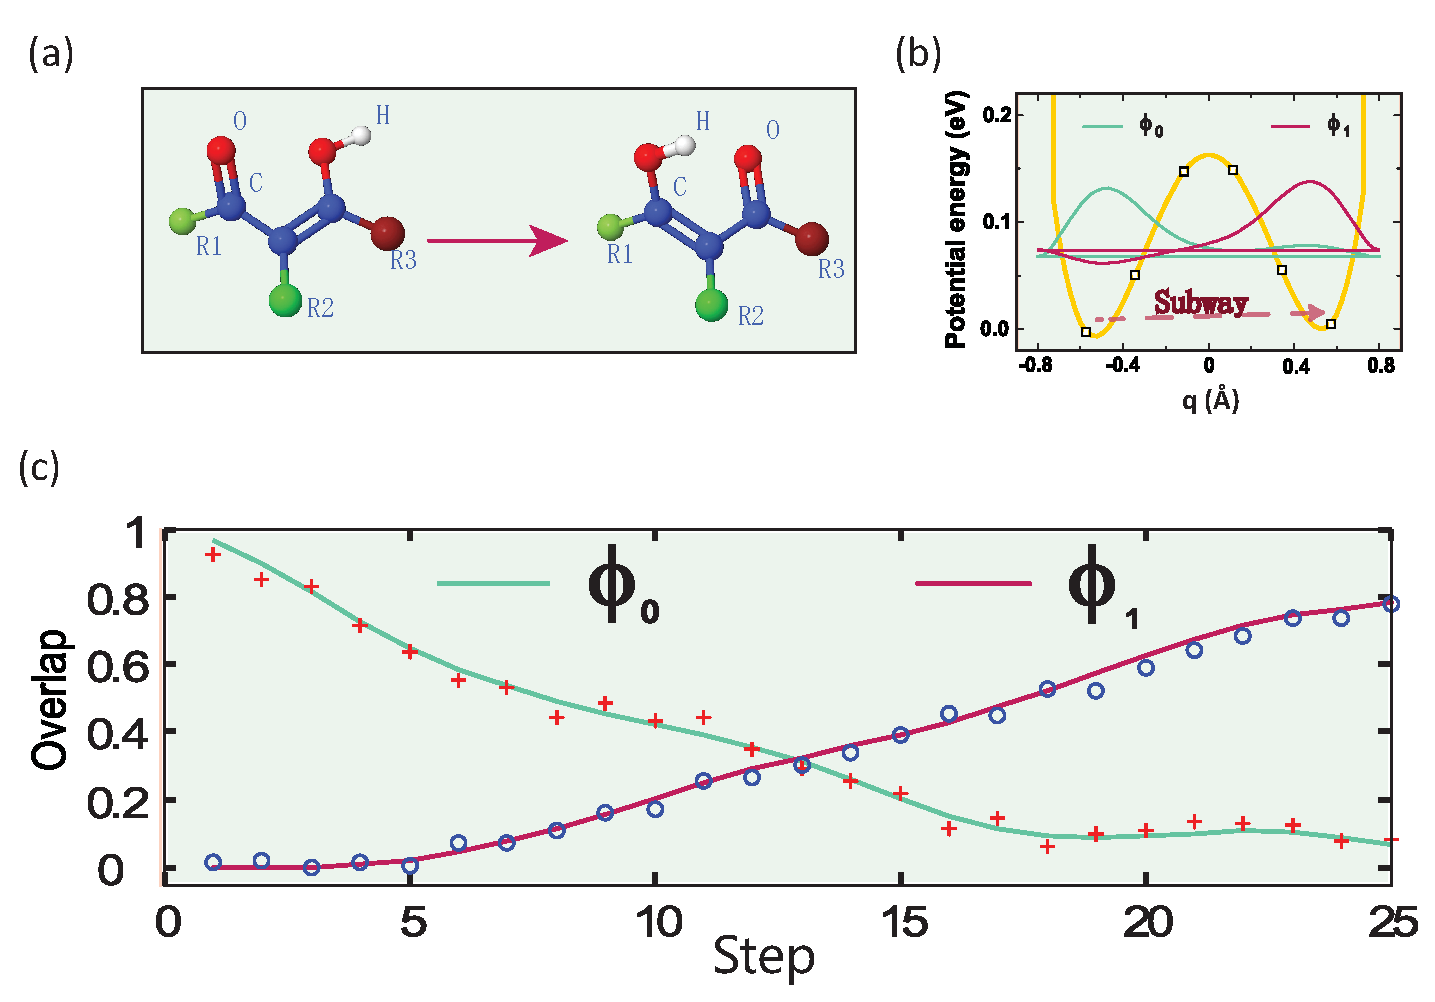
\includegraphics[width= 0.95\columnwidth]{fig4.eps}
\end{center}
\caption{(color online) (a) Isomerization reaction of nonsymmetric substituted malonaldehydes.
(b) Potential energy curve, together with the eigenfunctions of
    the ground (green) and the first excited (red) states.
    The "subway" represents the hydrogen tunneling approach.
(c) Measured probabilities of the reactant (ground) and product (first excited) states
    to give 25 snapshots of the reaction dynamics.
    The red plus symbols represent measured results of
    percentages of the reactant and the blue circles
    represent those of the product
    during the time evolution, both in agreement with
    the theoretical smooth curves. Reproduced from Lu \emph{et al.}, \emph{Phys. Rev. Lett.}, 2011, \textbf{107}, 020501.\cite{NMR_dynamic}}\label{fig4}
\end{figure}

This chemical isomerization reaction has been successfully exemplified
as the first experimental realization of
quantum simulation on chemical dynamics,
via a NMR quantum simulator.\cite{NMR_dynamic}
In our case, the reaction has one DOF, hence modeled
as an one-dimensional object, and described by qubits.
The laser-controlled dynamics is to the relocate hydrogen
of non-symmetric substituted malonaldehydes,\cite{Hydrogen-Subway}
as shown in Fig.\ref{fig4}(a).
For our implementation, we would like to discuss it in the following aspects:
initial state preparation of the molecule,
time evolution under the Hamiltonian operator,
and the measurement during and after the experiment,
followed by conclusions and future prospects.

Beginning with the state initialization,
the system Hamiltonian operator was originally time independent,
before the laser field. Nevertheless, to exploit
the ``hydrogen-subway'' effect under the influence of the laser field,
the new Hamiltonian needs to take the external electric field
into consideration. That is
\[H = T + V + E(t)\]
where $E(t)$ is the time-dependent lase-molecule interaction
and $T$ and $V$ are the time-independent kinetic and potential energy operators, respectively.
As illustrated in Fig.\ref{fig4}(b), the potential function $V$
is a double-well.
From the asymmetry of the shape, i.e.\
the difference in the well depths, it is assumed that
the initial state as the ground state of the system
is located in the left potential well,
whereas the product state as the first excited state
is in the right potential well.
The ``hydrogen-subway'' approach offers
an implementation of laser-controlled tunneling process
for the reaction to take place when the energy of the molecule is
below the barrier height.

Here, the kinetic energy operator is given as $T = p^{2} /(2m)$,
whilst the potential counterpart is described as
\be\label{potential}
 {V}=\frac{\Delta}{2q_0}(  q-q_0)+\frac{V^\ddag-\Delta/2}{q_0^4}(  q-q_0)^2(  q+q_0)^2
\ee
The laser field interaction is $E(t) = \mu\varepsilon(t)$,
where $\mu = eq$ is the dipole moment operator and $\varepsilon(t)$
represents the driving electric field:
\be
  \varepsilon(t)=\left\{
    \begin{array}{cc}
       \varepsilon_0\sin^2(\frac{\pi\, t}     {2s_1})         ;&\qquad   0\leq t\leq s_1\\
       \varepsilon_0                                        ;&\qquad   s_1<t<s_2\\
       \varepsilon_0\sin^2[\frac{\pi(t_{\!f}-t)}{2(t_{\!f}-s_2)}]   ;&\qquad   s_2\leq t\leq t_f
    \end{array}
  \right.
\ee
with $s_1=5\,$fs, $s_2=32.5\,$fs and $t_f=37.5\,$fs.

At the start of the simulation, $t = 0$,
the molecule should be prepared under the bare Hamiltonian $T + V$,
before the action of the laser field takes place.
To do this, we manipulated a pseudo-pure state from the
thermal equilibrium state, by applying a radio-frequency (rf)
pulse using the spatial average technique,\cite{spatial_averaging_1}
generated via the GRadient Ascent Pulse Engineering (GRAPE)
algorithm,\cite{GRAPE_1,NMR_readout,GRAPE_3} with a high fidelity of 0.995.
So far we have obtained the reactant state,
or the initial state, which was checked by a full state tomography
and then a fidelity test.
Following the definition of the fidelity $F(\rho_{1}, \rho_{2})\equiv \texttt{Tr}(\rho_1{\rho_2})/\sqrt{(\texttt{Tr}(\rho_1^2)\texttt{Tr}(\rho_2^2)}$,
we obtain $F[\rho_0, \rho_{\text{exp}}(0)]=0.950$,
where $\rho_0$ is the theoretical reactant state and
$\rho_{\text{exp}}(0)$ is the experimentally obtained initial state.
The tomographic results of them demonstrated
a high agreement between the theoretical reactant state
and the prepared one. Hence we were confident in moving onto the
time evolution of experiment from this initial state.

In the next step, we applied the propagator of the Hamiltonian,
$U$, to the system, which, in a small
enough time interval, follows
\[U(t+\delta t,t) \approx {e^{-iH(t+\delta t/2)\delta t}}\]
where $H = T + V + E(t)$.
The potential was quantized with eight discrete points,
represented by three qubits.
Undoubtedly, more elaborate discretization would
improve the precision of the simulation.
Nonetheless the availability of qubits limited our choices of
the number of quantized points.
To avoid the direct operation of the whole Hamiltonian,
the propagator is implemented by taking the Trotter formula,\cite{first_quantization_2,Trotter_1,Trotter_2}
\begin{align}\label{propagator}
 {U}(t+\delta t,t)\approx &\,
 e^{-i {V} \delta t/2} e^{-i {E} (t+\delta t/2)  \delta t/2}
 e^{-i {T} \delta t}   \nl & \times e^{-i {E} (t+\delta t/2)           \delta t/2}
 e^{-i {V} \delta t/2} .
\end{align}
Hence the propagator is decomposed into simple forms, consisting only of
unitary diagonal operators in either the position or momentum representation.
In a quantum computer, we could conduct QFT to realize transformations
between these two representations easily.

\iffalse

thus imposing all operators
into one representation,
relieving the burden of working in two representations.
Indeed, we did QFT to the $T$, kinetic energy operator,
and then by carrying out each operator
in order one iteration could be finished,
applying a rf pulse sequence to it.

\fi


Alternatively, an ancilla\cite{Polynomial_time_algorithm}
could be introduced to the loop.
However for the reason stated before,
extra qubits are required for the ancilla method,
which, again, were not available at the time of the experiment.
Instead, within low dimensions of the Hilbert space,
the GRAPE approach has proved to be
successful on an NMR simulator. Although its prospect is not
promising on high-dimensional density matrices,
it may be possible to produce a GRAPE pulse via feedback
learning control, exploiting the quantum evolution of
NMR system itself. Nonetheless, when the system scales up,
the ancilla approach is likely to provide a feasible solution
to simplify operators.

The final result at $t_f$
was obtained by iterating the loop of Eq.(\ref{propagator})
for 25 times with $\delta t=1.5\,$fs.
The limiting factor for the number of loops was at first
the operation time of applying rf pulse
for each operator and the decoherence time of the NMR system.
A solution to it is to combine a series of rf pulses for operators
in one loop
into one single rf pulse using the high fidelity GRAPE method,
which is a facile job for a 3-qubit system. With this
we were able to decrease the overall operation time,
as well as reduce the technical complexity,
while preventing serious decoherence effects
and other experimentally inevitable errors.
As a result of this, we achieve a high-fidelity end product.

For the purpose of observing the conversion from the reactant to
the product, the overlaps were measured between density matrices
during the experiment and those of the theoretical initial and final states.
This information was obtained
more simply by a diagonalization technique\cite{NMR_dynamic}
to measure the populations,
rather than the full state tomography
that demands much more resources.
The trend of overlap is shown in Fig.\ref{fig4}(c).

After the propagation, for the final product, we conducted
a close inspection of the discrepancy between the theory
and the experiment.
A full state tomography on the final state density matrix
is carried out to compare with the theoretical one,
in an eight dimensional Hilbert space.
Provided with the high fidelity of the GRAPE pulse (0.995),
the experimental final state and the theoretical one
agreed with each other to a great extent,
with fidelity of 0.957.
Furthermore, for the product state,
the experimental density matrix elements
and the theoretical ones are also consistent with high fidelity.

Therefore, the result in Fig.\ref{fig4}(c) achieved
from our quantum simulator demonstrates the time evolution of
reactant and product state probabilities.
The product-to-reactant ratio
rises gradually with time. A 77\%\ probability of
the product state is reached at the end of the simulation.

To summarize, an archetype chemical reaction driven by lasers
was successfully emulated by our 3-qubit NMR system.
Furthermore, as the operations of gates were merged via the GRAPE pulses,
the total number of operations was reduced.
We emphasize that the simulation time, 30\,ms, was considerably
shorter than our system spin decoherence time.
The insignificant difference
between the theory and the experiment may be caused by
the falseness of GRAPE pulses,
the inhomogeneity in rf pulses,
and the inconsistency in the static magnetic field.

\section{Conclusion and perspective}

In the paper we have reviewed the development of quantum simulation
towards quantum chemistry, in both theories and experiments.
Unlike the quantum computation algorithm which usually requires
thousands of qubits to display the superiority of polynomial
complexity of quantum computers,
quantum simulation architectures are expected to
surpass classical computers with just 30-100 qubits.
However, this requirement is still beyond the current
experimental equipment.
As proof-of-principle but pioneer experiments to
demonstrate the simulations of static molecular energy\cite{Alan_first}
and dynamical chemical reaction,\cite{Simulating_chemistry_computer}
the quantum simulation of hydrogen molecular ground state energies
in linear optics\cite{Optics_static} and NMR,\cite{NMR_static}
and the quantum simulation of an one-dimensional isomerization
chemical reaction in NMR,\cite{NMR_dynamic}
have exhibited elementary superiority
of quantum simulation as a powerful tool
to investigate quantum chemistry.
The main challenges of quantum simulation on quantum chemistry
for large systems are just the challenges
of building a practical quantum computer.
They include the preparation of initial states,
decomposition and application of arbitrary qubit evolutions,
measurement on the final states,
and ways to overcome noise and decoherence.
Although the current limitations of technique and hardware forbid us
to build a universal quantum simulator exceeding classical computers at present,
we propose in the following the possible improvements
in two directions of applications:
simulations of static molecular energies of larger molecules
and simulations of more complicated chemical reactions.

For larger molecules, since the simple and important hydrogen
molecule has been simulated successfully,
the next one taken into account could be the water molecule H$_2$O.
In the original scheme,\cite{Alan_first}
if choosing the minimal STO-3G basis set,
it is declared that simulating H$_2$O requires 8 qubits,
which is already available in some quantum systems.
Subsequently, a quantum algorithm to obtain the energy spectrum of a
molecule based on the multiconfigurational self-consistent field
is presented,\cite{water_static} with which the excited states are accessible.
As an example, the quantum simulation of the ground state
and the first singlet excited state of the water molecule
using the cc-pVDZ basis set\cite{ccpv} is demonstrated,
where 14 qubits are required on a quantum simulator. Recently, it is demonstrated that  for simulating the water molecule it just requires 6 qubits to obtain the energy spectrum instead of the ground state energy.\cite{water}
This could be an accessible object in the near future.

In dynamic chemical simulations,
the next potential step could be extending the system
into two dimensions. Obviously the Hamiltonian,
with its potential and kinetic energy operators,
would then be expressed in two dimensions.
If the system is quantized with a 16$\times$16 grid,
the required number of qubits is 8,
which would be feasible in near future.
However, if we apply the spilt-operator method\cite{Trotter_1,Trotter_2}
to the two dimensional problems, the number of quantum gates
would be hundreds or even thousands,
beyond the capacity of current quantum systems.
Nevertheless, it may be possible to make algorithmic progress
on other models, rather than the quantum circuit model.
For instance, topological quantum computing,\cite{topological_quantum_computing_1,topological_quantum_computing_2}
quantum walks,\cite{quantum_walks_1,quantum_walks_2,quantum_walks_3,quantum_walks_4}
and one-way quantum computing\cite{one-way_quantum_computing_1,one-way_quantum_computing_2,one-way_quantum_computing_3}
may boost the quantum chemical dynamics simulation of systems
beyond one dimension.

\section{Acknowledgement}

This work was supported by National Nature Science Foundation of
China (Grants Nos. 10834005, 91021005, and 21073171), the CAS, and the National Fundamental Research Program 2007CB925200.

%The \balance command can be used to balance the columns on the final page if desired. It should be placed anywhere within the first column of the last page.

%\balance

%If notes are included in your references you can change the title from 'References' to 'Notes and references' using the following command:
%\renewcommand\refname{Notes and references}

\footnotesize{
\bibliography{rsc} %your .bib file
\bibliographystyle{rsc} %the RSC's .bst file
}
\begin{thebibliography}{99}
%%%%%%%%%%%%%%%%%%%%%%%%%%%%%%%%%%%%%%%%%%%
\bibitem{Approximate}
T. Helgaker, P. Jorgensen and J. Olsen, 2002, \emph{Molecular Electronic Structure Theory}.

\bibitem{Feynman}
R. Feynman, \emph{Int. J. Theor. Phys.}, 1982, \textbf{21}, 467.

\bibitem{Lewensitein}
M. Lewenstein \emph{et al}., \emph{Adv. Phys.}, 2007, \textbf{56}, 243.



\bibitem{Quantum_simulator}
I. Buluta and F. Nori, \emph{Science}, 2009, \textbf{326}, 108.

\bibitem{Coherent_control}
V. Vedral \emph{et al}., \emph{Nature}, 2008, \textbf{453}, 1003-1049.

\bibitem{Lloyds}
S. Lloyd, \emph{Science}, 1996, \textbf{273}, 1073.

\bibitem{Alan_first}
A. Aspuru-Guzik, A. D. Dutoi, P. J. Love and M. Head-Gordon, \emph{Science}, 2005, \textbf{309}, 1704.

\bibitem{Qubits}
A. Friedenauer, H. Schmitz, J. T. Gl\"{u}kert, D. Porras and T. Sch\"{a}z, \emph{Nat. Phys.} , 2008, \textbf{4}, 757.

\bibitem{AQS_1}
M. Greiner, O. Mandel, T. Esslinger, T. W. H\"{a}sch and I. Bloch, \emph{Nature}, 2002, \textbf{415}, 39.

\bibitem{AQS_2}
E. Manousakis, \emph{J. Low Temp. Phys.}, 2002, \textbf{126}, 1501.

\bibitem{AQS_3}
A. Smirnov, S. Savel'ev, L. Mourokh and F. Nori, \emph{Eur. Phys. Lett.}, 2007, \textbf{80}, 67008.

\bibitem{DQS_1}
D. Abrams and S. Lloyd, \emph{Phys. Rev. Lett.}, 1997, \textbf{79}, 2586.

\bibitem{DQS_2}
R. Somma, G. Ortiz, J. E. Gubernatis, E. Knill and R. Laflamme, \emph{Phys. Rev. A}, 2002, \textbf{65}, 042323.

\bibitem{Nature_Rev}
T. Ladd, F. Jelezko, R. Laflamme, Y. Nakamura, C. Monroe and J. O'Brien, \emph{Nature}, 2010, \textbf{464}, 45.

\bibitem{Rep_Rev}
I. Buluta, S. Ashhab and F. Nori, \emph{Rep. Prog. Phys.}, 2011, \textbf{74}, 104401.

\bibitem{NMR_oscillator}
S. Somaroo, C. H. Tseng, T. F. Havel, R. Laflamme and D. G. Cory, \emph{Phys. Rev. Lett}., 1999, \textbf{82}, 5381-5384.

\bibitem{NMR_1}
X. H. Peng, J. F. Du and D. Suter, \emph{Phys. Rev. A}, 2005, \textbf{71}, 012307.

\bibitem{NMR_2}
C. Negrevergne, R.Somma, G.Ortiz, E. Knill and R. Laflamme, \emph{Phys. Rev. A}, 2005, \textbf{71}, 032344.

\bibitem{NMR_3}
X. Yang, A. M. Wang, F. Xu and J. Du, \emph{Chem. Phys. Lett}., 2006, \textbf{422}, 20.

\bibitem{NMR_4}
K. R. Brown, R. J. Clark and I. L. Chuang, \emph{Phys. Rev. Lett}., 2006, \textbf{97}, 050504.

\bibitem{NMR_5}
H. W. Chen, X. Kong, B. Chong, G. Qin, X. Y. Zhou, X. H. Peng and Jiangfeng Du, \emph{Phys. Rev. A}, 2011, \textbf{83}, 032314.

\bibitem{NMR_static}
J. F. Du, N. Y. Xu, X. H. Peng, P. F. Wang, S. F. Wu and D. W. Lu, \emph{Phys. Rev. Lett}., 2010, \textbf{104}, 030502.

\bibitem{NMR_dynamic}
D. W. Lu, N. Y. Xu, R. X. Xu, H. W. Chen, J. B. Gong, X. H. Peng and J. F. Du, \emph{Phys. Rev. Lett.}, 2011, \textbf{107}, 020501.

\bibitem{NMR_readout}
J. Baugh, J. Chamilliard, C. M. Chandrashekar, M. Ditty, A. Hubbard, R. Laflamme, M. Laforest, D. Maslov, O. Moussa, C. Negrevergne, M. Silva, S. Simmons, C. A. Ryan, D. G. Cory, J. S. Hodges and C. Ramanathan, \emph{Phys. in Can.}, 2007, \textbf{63}, 4.

\bibitem{NMR_review_1}
L. M. K. Vandersypen and I. L. Chuang, \emph{Rev. Mod. Phys}., 2005, \textbf{76}, 1037-1069.

\bibitem{NMR_review_2}
D. Cory \emph{et al.}, \emph{Fortschr. Phys}., 2000, \textbf{48}, 875.

\bibitem{Optics_review_1}
P. Kok, W. J. Munro, K. Nemoto, T. C. Ralph, J. P. Dowling and G. J. Milburn, \emph{Rev. Mod. Phys}., 2007, \textbf{79}, 797.

\bibitem{Optics_review_2}
J. L. O'Brien, \emph{Science}, 2007,  \textbf{318}, 1567-1570.

\bibitem{Optics_static}
B. P. Lanyon  \emph{et al}, \emph{Nat. Chem}., 2010, \textbf{2}, 106-111.

\bibitem{Optics_first}
E. Knill, R. Laflamme and G. J. Milburn, \emph{Nature}, 2001, \textbf{409}, 46-52.

%\bibitem{Ions_expt_1}
%A. Friedenauer, H. Schmitz, J. T. Glueckert, D. Porras and T. Schaetz, \emph{Nat. Phys}., 2008, \textbf{4}, 757-761.

\bibitem{Ions_expt_2}
R. Gerritsma, G. Kirchmair, F. Z\"{a}hringer, E. Solano, R. Blatt and C. F. Roos, \emph{Nature}, 2010, \textbf{463}, 68.

\bibitem{Ions_expt_3}
K. Kim, M. S. Chang, S. Korenblit, R. Islam, E. E. Edwards, J. K. Freericks,G. D. Lin, L. M. Duan and C. Monroe, \emph{Nature}, 2010, \textbf{465}, 560.

\bibitem{Ions_review_1}
R. Blatt and D. Wineland, \emph{Nature}, 2008, \textbf{453}, 1008-1015.

\bibitem{Ions_review_2}
J. I. Cirac and P. Zoller, \emph{Phys. Rev. Lett}., 1995, \textbf{74}, 4091.

\bibitem{Ions_review_3}
M. Johanning, A. F. Var\'{o}n and C. Wunderlich, \emph{J. Phys. B}., 2009, \textbf{42}, 154009.

\bibitem{Super_1}
M. Hofheinz \emph{et al.}, \emph{Nature}, 2009, \textbf{459}, 546.

\bibitem{Super_2}
L. DiCarlo \emph{et al.}, \emph{Nature}, 2009, \textbf{460}, 240.

\bibitem{Super_3}
F. Nori, \emph{Nat. Phys}., 2008, \textbf{4}, 589.

\bibitem{Super_4}
J. Q. You and F. Nori, \emph{Phys. Today}, 2005, \textbf{58}, 42.

\bibitem{Super_5}
J. Q. You, X. F. Shi, X. Hu and F. Nori, \emph{Phys. Rev. B}., 2010, \textbf{81}, 014505.

\bibitem{Super_10}
F. Nori, \emph{Science}, 2009, \textbf{325}, 689.

\bibitem{Super_6}
Garcia-Ripoll, J. J., E. Solano and M. A. Martin-Delgado, \emph{Phys. Rev. B}., 2008, \textbf{77}, 024522.

\bibitem{Super_11}
M. Neeley \emph{et al.}, \emph{Science}., 2009, \textbf{325}, 722.

\bibitem{Super_7}
B. G. Levi, \emph{Phys. Today}, 2009, \textbf{62}, 114.

\bibitem{Super_8}
J. Q. You and F. Nori, \emph{Nature}, 2011, \textbf{474}, 589.

\bibitem{Super_9}
P .D. Nation, J. R. Johansson, M. P. Blencowe and F. Nori, \emph{Rev. Mod. Phys.}, 2012, \textbf{84}, 1.

\bibitem{Dot_1}
R. Hanson and D. D. Awschalom, \emph{Nature}, 2008, \textbf{453}, 1043.

\bibitem{Dot_2}
T. Byrnes, P. Recher, N. Y. Kim, S. Utsunomiya and Y. Yamamoto, \emph{Phys. Rev. Lett.}, 2007, \textbf{99}, 016405.

\bibitem{Dot_3}
T. Byrnes, N. Y. Kim, K. Kusudo and Y. Yamamoto, \emph{Phys. Rev. B.}, 2008, \textbf{78}, 075320.

\bibitem{Cold_1}
I. Bloch, J. Dalibard amd W. Zwerger, \emph{Rev. Mod. Phys.}, 2008, \textbf{80}, 885.

\bibitem{Hydrogen}
A. Szabo and N. S. Ostlund, 1989,
\emph{Modern quantum chemistry:
Introduction to advanced electronic structure theory},
1st ed., Revised,
McGraw-Hill, New York.

\bibitem{Parr95}
R. G. Parr and W. T. Yang, \emph{Annu. Rev. Phys. Chem.},
1995, \textbf{46}, 701.

\bibitem{Kohn96}
W. Kohn, A. D. Becke, and R. G. Parr, \emph{J. Phys. Chem.},
1996, \textbf{100}, 12974.

\bibitem{Chelikowsky09}
J. R. Chelikowsky  \emph{et al.}, \emph{J. Comput. Theor. Nanosci}., 2009, \textbf{6}, 1247.

\bibitem{Goedecker99}
S. Goedecker, \emph{Rev. Mod. Phys.}, 1999, \textbf{71}, 1085.

\bibitem{Hung09}
L. Hung and E. A. Carter, \emph{Chem. Phys. Lett}., 2009, \textbf{475}, 163.

\bibitem{limit_1}
A. Dreuw and M. Head-Gordon, \emph{J. Am. Chem. Soc}., 2004, \textbf{126}, 4007.

\bibitem{limit_2}
B. G. Levine and T. J. Martinez, \emph{Ann. Rev. Phys. Chem}., 2007, \textbf{58}, 613.

\bibitem{limit_3}
P. A. Lee, N. Nagaosa and X. G. Wen, \emph{Rev. Mod. Phys}., 2006, \textbf{78}, 17.

\bibitem{Yang08}
A. J. Cohen, P. Mori-Sanchez and W. T. Yang, \emph{Science},
2008, \textbf{321}, 792.

\bibitem{Reaction_1}
H. Rabitz \emph{et al.}, \emph{Science}, 2000, \textbf{288}, 824; W. S. Warren, H. Rabitz and M. Dahleh, \emph{Science}, 1993, \textbf{259}, 1581.

\bibitem{Reaction_2}
S. A. Rice and M. Zhao, 2000, \emph{Optical Control of Molecular
Dynamics}, John Wiley, New York; M. Shapiro and P. Brumer, 2003,  \emph{Principles of the Quantum Control of
Molecular Processes}, John Wiley, New York.

\bibitem{DOF}
D. Wang, \emph{J. Chem. Phys}., 2006, \textbf{124}, 201105.

\bibitem{Hartree}
H. D. Meyer and G. A. Worth, \emph{Theor. Chem. Acc}., 2003, \textbf{109}, 251.

\bibitem{Prepare}
H. Wang, S. Ashhab and F. Nori, \emph{Phys. Rev. A}, 2009, \textbf{79}, 042335.

\bibitem{Simulating_chemistry_computer}
I. Kassal, J. D. Whitfield, A. Perdomo-Ortiz, M. H. Yung and A. Aspuru-Guzik, \emph{Annu. Rev. Phys. Chem}., 2011, \textbf{62}, 185-207.

\bibitem{Polynomial_time_algorithm}
I. Kassal, S. P. Jordan, P. J. Love, M. Mohseni and A. Aspuru-Guzik, \emph{Proc. Natl. Acad. Sci}., 2008, \textbf{105}, 18681.

\bibitem{first_quantization_1}
S. Wiesner, 1996, arXiv:quant-ph/9603028

\bibitem{first_quantization_2}
C. Zalka, \emph{Proc. Roy. Soc. A}, 1998, \textbf{454}, 313-322.
%\bibitem{pseudo-pure}
%D.G. Cory, M.D. Price, \&\ T.F. Havel, Physica D, \textbf{81}, 2152, (1998).

%\bibitem{logical_labeling_1}
%N. Gershenfeld and I.L. Chuang, Science, \textbf{275}, 350, (1997).


%\bibitem{logical_labeling_2}
%L.M.K. Vandersypen, C.S. Yannoni, M.H. Sherwood \&\ I.L. Chuang, Phys. Rev. Lett., \textbf{83}, 3085, (1999).

%\bibitem{temporal_averaging_1}
%E. Knill, I.L. Chuang and R. Laflamme, Phys. Rev. A, \textbf{81}, 5672, (1998).

%\bibitem{Adiabatic_1}
%E. Farhi, J. Goldstone, S. Gutmann, and M. Sipser, Quantum computation by adiabatic evolution. arXiv:quant-ph/0001106, (2000).

%\bibitem{Adiabatic_2}
%M. H. S. Amin, On the inconsistency of the adiabatic theorem. arXiv:0810.4335, (2008).

%\bibitem{Adiabatic_3}
%A. Messiah, Quantum Mechanics. Dover Publications, (1999).

%\bibitem{Adiabatic_4}
%D. M. Tong, Quantitative condition is necessary in guaranteeing the validity of the adiabatic approximation. Phys. Rev. Lett., \textbf{104}(12), 120401, (2010).

%\bibitem{Adiabatic_5}
%D. M. Tong, K. Singh, L. C. Kwek, \&\ C. H. Oh. Suffciency criterion for the validity of the adiabatic approximation. Phys. Rev. Lett., \textbf{98}, (15),150402-4, (2007).

\bibitem{Trotter_1}
D. Berry, G. Ahokas, R. Cleve and B. Sanders, \emph{Comm. Math. Phys}., 2007, 270:359.

\bibitem{Trotter_2}
N. Hatano and M. Suzuki, \emph{Lecture Notes in Physics}, 2005, \textbf{679}, 37-68.

\bibitem{PEA_1}
D. S. Abrams and S. Lloyd, \emph{Phys. Rev. Lett}., 1999, \textbf{83}, 5162-5165.

\bibitem{PEA_2}
A. Kitaev, 1995, arXiv:quant-ph/9511026.

\bibitem{PEA_3}
H. Wang, L. A. Wu, Y. X. Liu and F. Nori, \emph{Phys. Rev. A}, 2010, \textbf{82}, 062303.

\bibitem{PEA_4}
L. F. Wei and F. Nori, \emph{J. of Phys. A}, 2004, \textbf{37},4607.

\bibitem{Other_measuring_methods_1}
S. P. Jordan, \emph{Phys. Rev. Lett}., 2005, \textbf{95}, 050501.

\bibitem{Other_measuring_methods_2}
G. Ortiz, J. E. Gubernatis, E. Knill and R. Laflamme, \emph{Phys. Rev. A}, 2001, \textbf{64}, 022319.

\bibitem{Other_measuring_methods_3}
R. Somma, G. Ortiz, E. Knill and J. Gubernatis, \emph{Int. J. Quantum Inf}., 2003, \textbf{1}, 189.

\bibitem{Other_measuring_methods_4}
B. Terhal and D. DiVincenzo, \emph{Phys. Rev. A}, 2000, \textbf{61}, 022301.

\bibitem{Li}
Z. K. Li, M. H. Yung, H. W. Chen, D. W. Lu, J. D. Whitfield, X. H. Peng, A. Aspuru-Guzik and J. F. Du, \emph{Scientific Reports}, 2011, \textbf{1}, 88.

\bibitem{adiabatic}
A. Messiah, 1976, \emph{Quantum mechanics}, New York; T. Kato, {\it J. Phys. Soc. Jpn.}, 1950, \textbf{5}, 435.

\bibitem{factoring}
X. H. Peng, Z. Y. Liao, N. Y. Xu, G. Qin, X. Y. Zhou, D. Suter and J. F. Du, \emph{Phys. Rev. Lett.}, 2008, \textbf{101}, 220405.

\bibitem{inter1} J. F. Du, P. Zou, M. J. Shi, L. C. Kwek, J. W. Pan, C. H. Oh, A. Ekert, D. K. L. Oi and M. Ericsson, 2003, {\it Phys. Rev. Lett.} \textbf{91}, 100403.

\bibitem{inter2} X. H. Peng, X. W. Zhu, D. Suter, J. F. Du, M. L. Liu and K. L. Gao, 2005, {\it Phys. Rev. A.} \textbf{72},052109.

\bibitem{inter3} H. W. Chen, M. G. Hu, J. L. Chen and J. F. Du, 2009, {\it Phys. Rev. A.} \textbf{80},054101.

%\bibitem{Hydrogen} A. Szabo and N. S. Ostlund, 1996, \emph{Modern quantum chemistry}
%Dover Publications, New York.

\bibitem{Adiabatic_6} A. P. Young, S. Knysh and V. N. Smelyanskiy, 2005, {\it Phys. Rev.
Lett.} \textbf{101}, 170503.

\bibitem{Adiabatic_7} R. Schutzhold and G. Schaller, \emph{Phys. Rev. A}, 2006, \textbf{74}, 060304
(R).

\bibitem{Open_Dynamics} H. Wang, S. Ashhab and F.Nori, \emph{Phys. Rev. A}, 2011, \textbf{83}, 062317.


%DYNAMICS
\bibitem{QFT_1}
D. Coppersmith, 2002, arXiv:quant-ph/0201067.

\bibitem{ultracold}
E. Torrontegui, A. Ruschhaupt, D. Gu\'{a}ry-Odelin and J. G. Muga, \emph{J. Phys. B: At. Mol. Opt. Phys.}, 2011, \textbf{44}, 195302.

\bibitem{Hydrogen-Subway}
N. Do\u{s}li\'{c}, O. K\"{u}hn, J. Manz and K. Sundermann, \emph{J. Phys. Chem. A}, 1998, \textbf{102} (47), 9645-9650.

\bibitem{Keldysh_limit}
L. V. Keldysh, \emph{SoV. Phys. JETP}, 1965, \textbf{20}, 1307.


\bibitem{spatial_averaging_1}
D. G. Cory, A. F. Fahmy and T. F. Havel, \emph{Proc. Natl. Acad. Sci}., 1997, \textbf{94}, 1634.

\bibitem{GRAPE_1}
N. Khaneja \emph{et al}., \emph{J. Magn. Reson}., 2005, \textbf{172}, 296.


\bibitem{GRAPE_3}
C. A. Ryan, M. Laforest, J. C. Boileau and R. Laflamme, \emph{Phys. Rev. A,} 2008, \textbf{78}, 012328.

\bibitem{water_static}
H. Wang \emph{et al}., \emph{Phys. Chem. Chem. Phys}., 2008, 10, 5388-5393.

\bibitem{ccpv} T. H. Dunning, \emph{J. Chem. Phys}., 1989, 90, 1007.

\bibitem{water} H. Wang, S. Ashhab and F. Nori, 2011, arXiv:quant-ph/1108.5902v1.

\bibitem{topological_quantum_computing_1}
A. Kitaev, \emph{Ann. Phys.}, 2003, \textbf{303}, 2-30.

\bibitem{topological_quantum_computing_2}
C. Nayak, S. H. Simon, A. Stern, M. Freedman and S. D. Sarma, \emph{Rev. Mod. Phys}., 2008, \textbf{80}, 1083.

\bibitem{quantum_walks_1}
J. Kempe, \emph{Contemporary Physics}, 2003, \textbf{44}, 307.

\bibitem{quantum_walks_2}
 A. M. Childs, \emph{Phys. Rev. Lett.}, 2009, \textbf{102}, 180501.

\bibitem{quantum_walks_3}
N. B. Lovett, S. Cooper, M. Everitt, M. Trevers and V. Kendon, \emph{Phys. Rev. A,} 2010, \textbf{81}, 042330.

\bibitem{quantum_walks_4}
D. W. Lu, J. Zhu, P. Zhou, X. H. Peng, Y. H. Yu, S. M. Zhang, Q. Chen and J. F. Du, \emph{Phys. Rev. A,} 2010, \textbf{81}, 022308.

\bibitem{one-way_quantum_computing_1}
R. Raussendorf and H. J. Briegel, \emph{Phys. Rev. Lett.}, 2001, \textbf{86}, 5188.


\bibitem{one-way_quantum_computing_2}
R. Raussendorf, D. E. Browne and H. J. Briegel, \emph{Phys. Rev. A,} 2003, \textbf{68}, 022312.

\bibitem{one-way_quantum_computing_3}
 C. Y. Ju, J. Zhu, X. H. Peng, B. Chong, X. Y. Zhou and J. F. Du, \emph{Phys. Rev. A,} 2010, \textbf{81}, 012322.




\end{thebibliography}

\end{document}
